\subsection{Dataset}
\label{sec:dataset}

\subsection{Benchmark Methods}
\label{sec:benchmark}

\subsection{Results}
\label{sec:res}

\subsection{Discussion}

%For evaluating the performance of the proposed algorithm, we use the dataset reported by the authors in \cite{beeman2011measuring}. Furthermore, the estimated glomerular number is compared against the results obtained using the MRI segmentation used in \cite{beeman2011measuring}, acid maceration, and stereological methods. We now briefly describe the procedure for obtaining the images in the dataset. Additional details on the materials and methods can be found in \cite{beeman2011measuring}. Cationic ferritin was synthesized and male Sprague-Dawley rats, weighing between 215 and 245 g, were given three intravenous bolus doses. Kidneys were perfused and fixed via transcardial perfusion of PBS \textit{(expand???)} followed by $10\%$ neutral buffered formalin, then resected and stored in glutaraldehyde. The perfused left kidneys were imaged in glutaraldehyde on a Varian 19T 89-mm-bore NMR (Varian, Palo Alto, CA), equipped with a DOTY 3-axis imaging probe and a gradient with a maximum strength of 300 G/cm (DOTY Scientific, Columbia, SC). Scans were acquired with a 3D gradient echo (GRE) sequence with echo time/repetition time $= 7/40$ ms and a resolution of $62 \times 62 \times 78 \mu$m. Total scan time was 6 hours/kidney.
%
%
%Labeled glomeruli in the 3D MRI data set can be counted using the method described in \cite{beeman2011measuring}. Using bicubic interpolation, images in the data set were resized and the spatial resolution was changed to $31 \times 31 \times 62 \mu$m. Spatial signal magnitude gradients were computed to identify significant spatial changes in signal magnitude throughout the volume. Only voxels exceeding a threshold on the signal magnitude difference were included for the subsequent operations. Following this, regional minima were located in these areas using an upper signal magnitude threshold. Regions in the image considered to be glomeruli were then labeled based on morphological thresholds. Note that, here it is assumed that a glomerulus is approximately spherical. Finally, the watershed transform \cite{} was computed on these regions to distinguish individual glomeruli where signal overlap of multiple glomeruli might occur.
%
%\begin{figure}[t]
%\begin{minipage}[b]{1.0\linewidth}
%  \centering
%  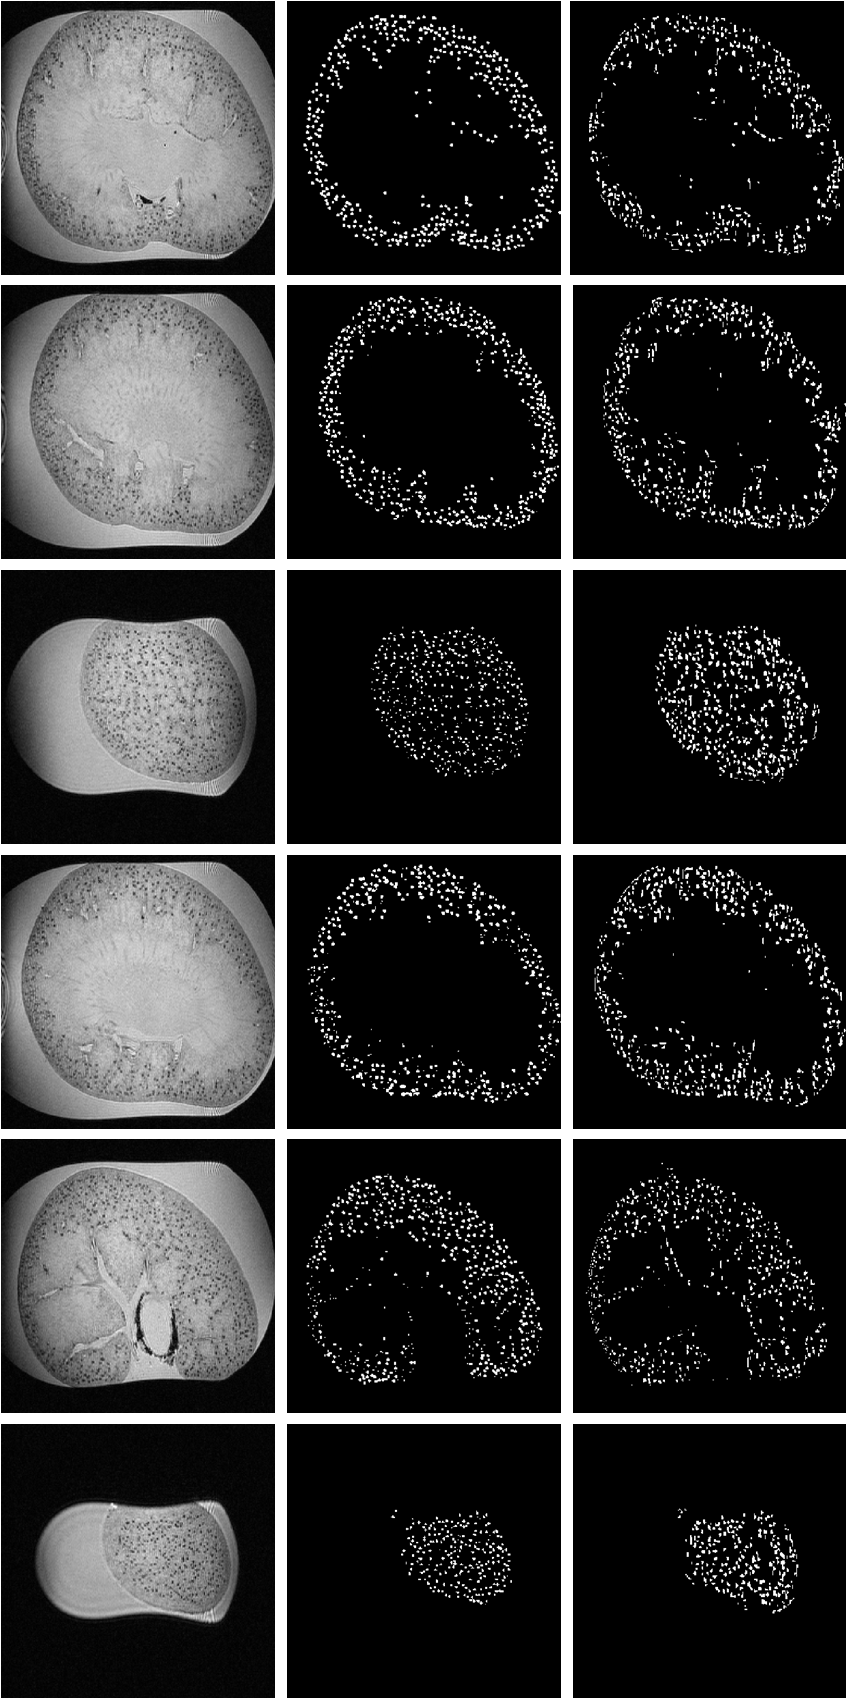
\includegraphics[width=8cm]{results.png}
%\end{minipage}
%\caption{Segmentation results for a sample set of MRI images obtained using the proposed algorithm. (Left-Right) Original kidney image with reduced intensities at glomeruli locations; ground truth image with manually labeled glomeruli regions; segmentation obtained using the approach described in Section \ref{sec:count}.}
%\label{Fig:res}
%\end{figure}
%
%\begin{table*}[t]
% \renewcommand{\arraystretch}{1.4}
%\centering
%\caption{Glomerular count obtained using acid maceration, stereology, and the MRI techniques, for three different datasets. Each dataset consisted of $192$ images and total glomerular count is shown. In addition, the total time taken, in seconds, to process each dataset using the proposed algorithm is shown.}
%\begin{tabular}{|c|c|c|c|c|c|}
%\hline
%\textbf{Dataset}&\textbf{MRI Number \cite{beeman2011measuring}}&\textbf{Maceration Number}&\textbf{Stereology Number}&\textbf{Proposed Algorithm}&\textbf{Total Time Taken (s)} \\
%\hline
%\hline
%Rat A&$32,789$&$27,504$&$34,504$&$33,884$&$41.1$ \\
%Rat B&$35,203$&$31,190$&$35,421$&$34,335$&$42.4$ \\
%Rat C&$31,772$&$31,075$&&$32,117$&$44.9$ \\
%Rat D&$39,482$&$33,321$&&$34,765$&$40.3$ \\
%Rat E&$29,682$&$31,478$&&$35,208$&$46.6$ \\
%\hline
%Mean&$33,786$&$30,914$&$34,963$&$34,062$&$43.1$ \\
%STD&$3,753$&$2,112$&$648$&$1193$&$2.6$\\
%\hline
%\end{tabular}
%\label{Table:count}
%\end{table*}
%
%
%In this section, we report the results obtained using the proposed algorithm, in comparison to the benchmark technique with MRI images: acid maceration and stereology methods. The evaluation was carried out with three different subjects (\textit{Rat A}, \textit{Rat B}, and \textit{Rat C}) and the glomerular count for the MRI based approaches were obtained from $192$ slices. Note that the results reported for the proposed algorithm were obtained using only $2$-D slices. \textit{(We may get a question, why we did not do 3D. If we are not planning to do 3D, we must write a good reason, because all our comparisons are with 3D)} For obtaining the discriminant mapping, $5$ ground truth images were used and patches of size $5 \times 5$ were extracted. Using the ground truth labels, a training set containing $7,500$ positive and $7,500$ negative example patches was generated. The patches were normalized, and the four $\ell_1$ graphs were constructed with the sparsity penalty $\lambda$ fixed at $0.2$. The number of reduced dimensions $d$ was fixed at $10$ and the mapping $\mathbf{V} \in \mathbb{R}^{25 \times 10}$ was obtained using the algorithm described in Figure \ref{Fig:train}. For each image in the evaluation \textit{(or test???)} dataset, the normalized $5 \times 5$ patches were projected onto the discriminant directions, and K-means clustering was performed to identify the glomeruli. Finally, the number of independent regions was counted and reported as the glomerular number.
%
%Figure \ref{Fig:res} illustrates the segmentation obtained for a set of test \textit{(or validation??? Technically, we do not know the glomeruli regions for test images)} images, using the proposed algorithm. In each case, both the original and ground truth images are shown for comparison. Clearly, the proposed algorithm provides impressive \textit{(too strong of a word)} results in determining the glomerular regions and the glomerular count obtained using the proposed algorithm is comparable to count obtained with manual labeling. The glomerular counts for the three evaluation \textit{(test???)} datasets are shown in Table \ref{Table:count}. The results obtained using the proposed method are comparable to the stereology results, and the standard deviation is comparatively lower \textit{(Table I does not say so)}. Another important advantage of the proposed scheme is its low computational complexity, which is evident from the time reported in Table \ref{Table:count}. The algorithm was implemented using MATLAB R2012a on a 2.8GHz, Intel i7 desktop.
%
%
